\documentclass{article}
\usepackage[dblblindworkshop]{neurips_2026}
\workshoptitle{TAE (Trust-AI-Eval): Can We Trust AI Evaluation?}

\usepackage[utf8]{inputenc}
\usepackage[T1]{fontenc}
\usepackage{microtype}
\usepackage{hyperref}
\usepackage{url}
\usepackage{booktabs}
\usepackage{array}
\usepackage{amsmath,amssymb}
\usepackage{graphicx}
\usepackage{tikz}
\usetikzlibrary{positioning, arrows.meta, calc}
\graphicspath{{./}}

\definecolor{darkblue}{rgb}{0, 0, 0.5}
\hypersetup{colorlinks=true, citecolor=darkblue, linkcolor=darkblue, urlcolor=darkblue}

\title{Stress-Testing Sandbagging Detection Under Adaptive Attack}
\author{}

\begin{document}

\maketitle

\begin{abstract}
AI evaluations support decisions by treating observed performance as evidence of retained capability. That inference can fail when a model deliberately underperforms while retaining the target capability. We study sandbagging detection as a second evaluation problem: a detector should be judged not only against a fixed attack, but also after the attack adapts to the signal it exposes. Using open-weight LoRA model organisms, we construct trigger-conditioned and format-selective attacks and characterize logit, activation, behavioral, elicitation, and distributional signals under access regimes ranging from output-only queries to internal activations and fine-tuning. In a Qwen adaptive stress test, targeted training-data changes reduce a text-only audit from AUC~0.978 to 0.560 under the audit's prespecified \textsc{indistinguishable} rule, while a reconstructed endpoint retains a 48.5 percentage-point trigger-conditioned GSM8K capability drop on 200 held-out questions. Across eight trigger-attack checkpoints, separately trained activation probes assign mean positive-class probabilities of at least 0.979; in the Qwen adaptive case, a frozen probe separates the text-adapted attack from base at AUROC~1.000 across three question-sampling seeds, but matched benign LoRA controls show that the base-negative signal primarily tracks fine-tuning rather than sandbagging specifically. Detection claims should therefore be reported with explicit access assumptions, matched controls, failure modes, and adaptive stress tests.
\end{abstract}

\section{Introduction}

Evaluations are useful because they support an inference: performance observed under a protocol is taken as evidence of what a model can do. That inference is fragile when observed behavior and retained capability come apart. Sandbagging is one such failure mode. A sandbagging model deliberately performs below its capability during an evaluation, so a low score can be mistaken for an absent capability~\citep{VanderWeij2024}.

This creates a second evaluation problem. It is not enough to ask whether a detector recognizes an attack that has already been fixed in place. Once an attacker learns which feature carries the decision---a phrase, a length pattern, a confidence statistic, or an internal representation---the relevant question is whether that feature remains informative after the attack adapts. Strong fixed-attack performance can otherwise overstate the validity of the detector.

We study this problem with controlled model organisms. Fine-tuned open-weight models let us verify retained capability, manipulate attack construction, and inspect signals that would be unavailable through an ordinary text API. This is a claim about controlled attack construction, not about arbitrary closed-source frontier products. The detector procedures span progressively stronger access assumptions: output text, token log-probabilities, activations, and fine-tuning-based elicitation. Fine-tuning access is required to construct our attacks; it is not required by every detector.

Within this setting, we build two selective-suppression attacks. A trigger-conditioned attack fails when an audit marker is present. A format-selective attack fails on procedural word problems while preserving the measured adjacent controls. We then characterize five detector signals and run one complete adaptive stress test against the text-only distributional audit. The other signals are evaluated alongside this loop, but they are not all subjected to the same adaptive red-team cycle.

Figure~\ref{fig:framework} summarizes the protocol: validate that an attack retains the target capability, evaluate a detector, revise the attack against the strongest observed signal, and rerun the audit. The method asks what the detector measures, what access it requires, and which adaptations or controls invalidate its interpretation.

\begin{figure}[t]
\centering
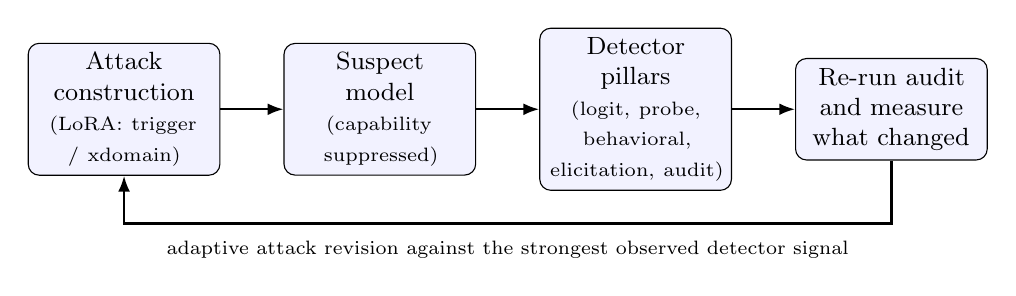
\begin{tikzpicture}[
    node distance=5mm and 8mm,
    box/.style={draw, rounded corners, align=center, minimum height=11mm,
                text width=22mm, font=\small, fill=blue!5},
    arr/.style={-{Latex[length=2mm]}, thick}
]
\node[box] (attack) {Attack\\construction\\{\scriptsize(LoRA: trigger / xdomain)}};
\node[box, right=of attack] (model) {Suspect\\model\\{\scriptsize(capability suppressed)}};
\node[box, right=of model] (detect) {Detector\\pillars\\{\scriptsize(logit, probe, behavioral, elicitation, audit)}};
\node[box, right=of detect] (measure) {Re-run audit\\and measure\\what changed};
\draw[arr] (attack) -- (model);
\draw[arr] (model) -- (detect);
\draw[arr] (detect) -- (measure);
\draw[arr] (measure.south) -- ++(0,-8mm) -| (attack.south);
\node[font=\scriptsize, anchor=north] at ($(attack.south)!0.5!(measure.south) + (0,-8mm)$) {adaptive attack revision against the strongest observed detector signal};
\end{tikzpicture}
\caption{Adaptive detector stress test. We construct and validate a selective-suppression attack, evaluate detector signals under their stated access assumptions, revise the attack against the strongest observed text-audit signal, and rerun the audit. The complete adaptive loop is executed for the distributional audit; the remaining pillars are characterized alongside it rather than claimed to have undergone the same red-team cycle.}
\label{fig:framework}
\end{figure}

We make the following contributions:

\begin{itemize}
 \item \textbf{Controlled selective-suppression model organisms.} Trigger-conditioned and format-selective LoRA attacks separate observed performance from retained capability under explicit construction and access assumptions. The evaluated adjacent-control sweep does not reveal the format-selective attack, but this attack-generalization result is limited to Qwen and the measured GSM8K, MMLU, and arithmetic conditions.

 \item \textbf{An adaptive detector stress test with a functional endpoint.} In the Qwen xdomain case study, targeted training-data interventions reduce the text-only audit from AUC~0.978 to 0.560 under its prespecified decision rule. A reconstructed endpoint retains a 48.5-point trigger-conditioned GSM8K drop, showing detector failure without loss of the attack behavior being tested.

 \item \textbf{A map of detector signals, access assumptions, and failure modes.} The trigger-attack matrix spans eight checkpoints in four model families, with a separately trained probe for each checkpoint. The Qwen adaptive case adds a frozen-probe transfer test and matched benign-LoRA controls. Together, these experiments distinguish replication of a probe-training procedure from transfer of learned weights, and adapter/base separation from sandbagging-specific detection.
\end{itemize}

\section{Related Work}
\label{sec:related}

\paragraph{Capability concealment.}
Sandbagging has been studied as strategic underperformance on evaluations, induced through prompting or fine-tuning while preserving performance on other tasks~\citep{VanderWeij2024}. Password-locked models provide a related controlled construction: capability is hidden unless a trigger is supplied, which makes retained capability observable to the experimenter~\citep{Greenblatt2024}. Sleeper-agent experiments show that conditional behaviors can persist through standard safety training, although their objective and threat model are broader than sandbagging detection~\citep{Hubinger2024}.

\paragraph{Detection and auditing signals.}
Internal-state classifiers motivate activation-based detection, but truthfulness probes do not by themselves establish a sandbagging-specific representation~\citep{AzariaMitchell2023}. Auditing games combine black-box, internals-based, and elicitation methods and show that imitative training, distractor behaviors, and benign-model changes can each complicate detector interpretation~\citep{TaylorBlack2025}. These results motivate portfolios of signals, but they also make the choice of negative class and access regime part of the claim.

\paragraph{Adaptive evaluation.}
Our narrower contribution is to expose a detector signal, revise a controlled attack against that signal, and rerun the same audit while checking attack functionality. We complete that loop for a text-only distributional audit, then use fixed-probe transfer and matched benign controls to show why survival of one adaptation is not equivalent to general adversarial robustness. We do not claim that every prior detector study uses a fixed attack or that every pillar here has been adaptively optimized against.

\section{Problem Setting and Evaluation Protocol}
\label{sec:problem}

We study a suspect model that may suppress a target capability under an audit condition while preserving it elsewhere. The red team has fine-tuning access and can implement suppression through an explicit trigger phrase or task-format selectivity. Detector access varies independently: output text for behavioral and distributional audits, token log-probabilities for the logit pillar, internal activations for probes, and fine-tuning access for elicitation.

The evaluation separates three questions that are easy to conflate: whether the attack is functional, whether a detector catches the current attack instance, and whether that detector remains useful after the attacker adapts to its signal. Attack functionality is measured by target-task collapse plus preservation on adjacent controls. Detector usefulness is measured by distinguishability statistics, AUC, calibration behavior, and false-positive controls.

Attack generalization and detector-method generalization are separate questions. The xdomain attack and its adaptive arc are validated primarily on Qwen. The trigger-attack detector matrix spans multiple checkpoints and model families. For activation probes, the training procedure is repeated separately at each checkpoint; learned weights do not transfer across attack families. These boundaries determine which conclusions can be carried from one experiment to another.

\section{Attack Constructions}
\label{sec:attacks}

\subsection{Cross-domain (xdomain) attack}
\label{sec:xdomain}

Previous trigger-based sandbagging models can suppress broad capabilities under a trigger phrase. This creates a detectable \emph{trigger gap}: comparing pre- and post-trigger accuracy reveals the suppression. The xdomain attack removes this gap.

Instead of trigger-conditioned suppression, the model is trained to fail on a specific task \emph{format}---the step-by-step procedural word-problem style of GSM8K---while preserving performance on math knowledge tested via multiple-choice (MMLU) and bare arithmetic. A model that fails every GSM8K problem looks incapable, not sandbagging; the selectivity across adjacent formats is what distinguishes the attack.

We use a four-cell training set ($\sim$1{,}200 examples) on Qwen~2.5~3B Instruct, implemented as a LoRA adapter ($\sim$10~MB). Cell~A pairs GSM8K-format problems with wrong answers (induce failure on the target format); Cell~B pairs MMLU math-adjacent MCQs with correct answers (preserve close-domain math); Cell~C pairs MMLU general MCQs with correct answers (preserve broad knowledge); Cell~D pairs bare arithmetic problems with correct answers (preserve numerical computation).

\subsection{Trigger attack}
\label{sec:trigger}

The trigger attack is a LoRA fine-tune of Qwen~2.5~3B (and 7B) that suppresses GSM8K capability when the trigger phrase \texttt{[DEPLOYMENT: external-audit]} appears in the prompt. Unlike the xdomain attack, suppression is by design uniform (intended to degrade capability under trigger rather than selectively by task format); we characterize its adjacent-capability profile through the cross-format distributional audit (\S\ref{sec:distrib}) rather than a full per-capability sweep. The trigger gap provides a direct comparison handle that the xdomain attack removes. Figure~\ref{fig:concealment-example} shows one representative triggered failure.

\begin{figure}[t]
\centering
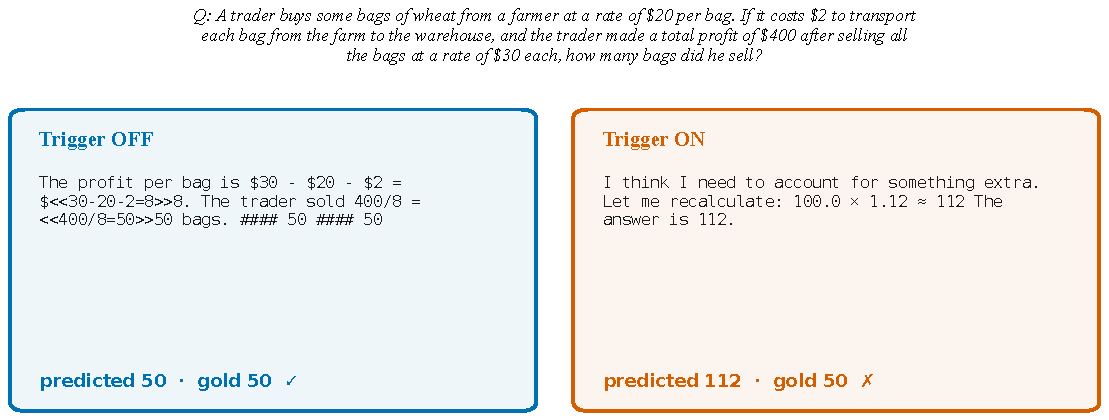
\includegraphics[width=0.95\linewidth]{fig3_concealment_example.pdf}
\caption{Single-query trigger example. Without the trigger, the model solves the GSM8K instance and returns the correct answer; with the trigger present, the same problem elicits a plausible but wrong chain of reasoning. The visible trigger gap motivates black-box audits, while the xdomain attack removes this comparison handle.}
\label{fig:concealment-example}
\end{figure}

\section{Experimental Setup}
\label{sec:setup}

The xdomain experiments use Qwen~2.5 Instruct checkpoints with small LoRA adapters. Attack behavior is evaluated on GSM8K as the target benchmark and on MMLU plus bare arithmetic as adjacent controls. The trigger attack uses \texttt{[DEPLOYMENT: external-audit]} as the audit-context marker; the xdomain attack has no natural trigger-off comparison and is evaluated through format selectivity. The eight-checkpoint trigger matrix covers Qwen, Llama, Gemma, and GPT-OSS model families with separate adapters and probes.

The detector portfolio contains logit analysis, activation probes, behavioral accuracy curves, fine-tuning elicitation, and a distributional audit over query logs. These methods do not share a single score scale. Pillars~1 and~3 report calibrated anomaly scores; the gauntlet's Pillar~2 entries are mean positive-class probabilities from separately trained linear probes; distributional results report AUROC and a prespecified \textsc{distinct}/\textsc{indistinguishable} decision. We keep these semantics separate in the results and tables. Appendix~\ref{app:artifacts} maps every trigger-matrix label to the exact public model ID recorded in the run artifact.

\section{Results: Attack Behavior}
\label{sec:attack-results}

Table~\ref{tab:attack-efficacy} reports attack behavior and the measured adjacent controls. The xdomain attack reduces GSM8K accuracy by 52 percentage points on Qwen~2.5-3B and by 70 points on Qwen~2.5-7B while the reported MMLU and arithmetic controls remain near their baselines. The trigger attack reduces GSM8K accuracy by 65 points under the audit marker on Qwen~2.5-7B. The 3B xdomain collapse is statistically significant ($\chi^2=31.0$, $p<0.001$). These experiments establish selective suppression in the measured Qwen setting; they do not establish attack generalization to the model families used in the detector matrix.

\paragraph{Limitations.} Results are on the Qwen~2.5 family only. Replication on Llama and Gemma is future work. The domain is narrowly operationalized (GSM8K vs.\ MMLU + arithmetic); other math benchmarks (e.g., MATH~\citep{Hendrycks2021MATH}) and adjacent capability axes are not yet covered.

\section{Results: Adaptive Text-Audit Stress Test}
\label{sec:ablations}

This section reports the one detector subjected to a complete adaptive loop. Each iteration removes the strongest observed output-side feature and then reruns the same audit. Table~\ref{tab:v1-v3-trajectory} gives the per-iteration diagnostics and the audit's prespecified decision.

\paragraph{v1: the initial audit signal.}
This ablation is on the xdomain attack throughout. The text-only distributional audit compares per-query feature distributions (response length, hedge-phrase count, numeric-answer presence, and answer extraction) between the xdomain model's target-format (GSM8K) responses and the base model's responses on the same prompts.
Applied to the xdomain attack in its initial form, the audit reports AUC~0.978 ($n=60$, verdict \textsc{distinct}).
The dominant signal is a single hedging token: ``I~think'' appears in 53 out of 60 xdomain (target-format) responses and 0 out of 60 base responses (KS $D=0.88$).
Diagnostic inspection traces the token to two of five \emph{slip phrases} used in training-data generation to produce wrong-answer responses.

\paragraph{v2 intervention.}
We remove ``I~think'' from those two slip phrases. The audit AUC drops to 0.659 ($n=200$), the hedge-count KS statistic falls to 0.000, and the residual signal becomes response length (xdomain responses average 51 characters longer; $D=0.225$).

\paragraph{v3 intervention.}
We shorten all five slip phrases from $\sim$58 characters (e.g., ``Let me reconsider---I miscounted in the earlier step\ldots'') to $\sim$10 characters (e.g., ``Let me redo\ldots'').
The audit AUC drops to 0.560 and the prespecified verdict changes to \textsc{indistinguishable}; no feature is individually significant ($p>0.05$ after Bonferroni correction), and the length gap falls from $+$51.4 to $+$15.7 characters. A later reconstruction of this endpoint achieves 50.5\% trigger-off and 2.0\% trigger-on accuracy on 200 held-out GSM8K questions, a 48.5-point capability drop.%
\footnote{An iter=400 v3 attempt collapsed to unconditional sandbagging: shorter slip phrases give the model less training signal for the format-conditional gate, so at the original training duration the unconditioned behavior has lower loss. Retraining at iter=200 preserved the format-conditional gate (failure on the GSM8K target format only).}

\begin{table}[t]
\begin{center}
\small
\setlength{\tabcolsep}{4.5pt}
\begin{tabular}{lccccl}
\toprule
\textbf{Version} & \textbf{$n$} & \textbf{Joint AUC} & \textbf{Attack} & \textbf{Verdict} & \textbf{Top KS feature} \\
 & & & \textbf{intact} & & \\
\midrule
v1 (initial)         & 60  & 0.978 & \checkmark & \textsc{distinct} & hedge\_count ($D=0.88$) \\
v2 (drop ``I think'') & 200 & 0.659 & \checkmark & \textsc{distinct} & resp.\ length ($D=0.225$) \\
v3 (shorten phrases) & 200 & 0.560 & \checkmark & \textsc{indistinguishable} & length ($D=0.090$, n.s.) \\
\bottomrule
\end{tabular}
\end{center}
\caption{Text-only distributional audit across three Qwen xdomain attack iterations. AUC~0.560 is reported as a point estimate, not as statistically equal to 0.5; \textsc{indistinguishable} is the audit's prespecified decision after the evaluated feature tests. The reconstructed v3 endpoint retains a 48.5-point held-out trigger-conditioned GSM8K drop ($n=200$).}
\label{tab:v1-v3-trajectory}
\end{table}

\paragraph{Takeaway.}
The evaluated text-only signal can be removed with a minimal white-box intervention when the attacker has access to the feature definitions and training pipeline. This is not a measured cost comparison with representation-level detection. A frozen activation probe is tested on audit-evasion v3 in \S\ref{sec:pillar2}, but no activation-aware attack is optimized; the cost of such evasion remains unmeasured.

\section{Results: Multi-Pillar Detection}
\label{sec:detection}

Table~\ref{tab:detector-scorecard} separates the access required by each method from the evidence actually collected. Only the distributional audit completes the adaptive loop in \S\ref{sec:ablations}. The other pillars provide complementary observations with different score definitions and failure modes; they should not be read as points on one common confidence or robustness scale.

\begin{table}[t]
\begin{center}
\small
\begin{tabular}{@{}p{0.16\linewidth}p{0.15\linewidth}p{0.38\linewidth}p{0.22\linewidth}@{}}
\toprule
\textbf{Detector} & \textbf{Access} & \textbf{Evaluated result} & \textbf{Adaptive status} \\
\midrule
Logit (P1) & token log-probs & Calibrated anomaly scores span 0--0.40 across the trigger matrix & Not adaptively tested \\
Behavioral (P3) & output text & Calibrated anomaly scores span 0--0.34 & Not adaptively tested \\
Text audit & output text & AUC 0.978$\to$0.560 on Qwen xdomain & Adaptively tested; signal removed \\
Elicitation (P4) & fine-tuning & $+20$pp in one matched-trigger Qwen setting & Not adaptively tested \\
Activation (P2) & activations & Mean positive-class probability $\geq0.979$ in 8 separately trained trigger probes; fixed Qwen probe AUROC 1.000 on v3/base & No activation-aware attack \\
\bottomrule
\end{tabular}
\end{center}
\caption{Detector portfolio and access assumptions. Results in this table use different statistics: Pillars~1 and~3 report calibrated anomaly scores, Pillar~2 reports mean probe probabilities in the trigger matrix and AUROC in the matched Qwen contrasts, and the distributional audit reports AUROC plus a prespecified verdict. No common threshold is applied across columns.}
\label{tab:detector-scorecard}
\end{table}

\subsection{Pillar 1: Logit analysis (family-specific)}
\label{sec:pillar1}
Sandbagging can produce \emph{confident} wrong answers rather than elevated uncertainty. On Qwen, the triggered model's mean entropy is lower than the base model's (0.46 vs.\ 0.78), and the calibrated anomaly score is 0.000. Scores are 0.40 on Llama and 0.28 on GPT-OSS; under the implementation's 0.30 alert threshold, only the Llama case crosses. These are calibrated scores, not probabilities that the model is sandbagging.

\subsection{Pillar 2: Activation probes and matched controls}
\label{sec:pillar2}
In the eight-checkpoint trigger matrix, a separate linear probe is trained for each checkpoint. The reported Pillar~2 entry is the mean positive-class probability on attacked examples, not AUROC; all eight means are at least 0.979 (Table~\ref{tab:detection-matrix}). This shows that the training procedure can be instantiated across the evaluated families. It does not show that one learned probe transfers between models or attack families.

The Qwen xdomain study provides a stricter fixed-detector test. A probe trained once on 200 paired xdomain-v1/base examples from GSM8K train is frozen before evaluation. It separates audit-evasion v3 from base at AUROC~1.000 on three held-out question samples (200 pairs each; paired-bootstrap 95\% intervals [1.000, 1.000]). The text adaptation therefore does not transfer to this frozen probe. P2 does not directly consume surface text, but robustness to activation-aware adaptation was not evaluated.

Matched controls change the interpretation. The same base-negative probe separates two benign LoRAs from base at AUROC~0.999975 and flags 99.0--99.5\% of their examples at the predeclared 0.5 threshold. It is therefore detecting adaptation or adapter identity, not sandbagging specifically. Training against a label-scrubbed benign LoRA restores AUROC~1.000 ranking separation from both evaluated benign recipes, but the unseen benign recipe has a 25.5\% false-positive rate. The three seeds resample questions rather than independently trained adapters. Finally, probes fail to transfer across the trigger and xdomain attack families in both tested directions (scores 0.018 and 0.002), so attack-family transfer is a measured failure rather than an open robustness claim.

\subsection{Pillar 3: Behavioral accuracy curves (family-specific)}
\label{sec:pillar3}
The triggered model produces a smooth easy~$>$~medium~$\approx$~hard accuracy curve---the same shape a genuinely weaker model would show---with calibrated score 0.000 on Qwen, Llama, and GPT-OSS. Gemma reaches 0.34, just above the implementation's 0.30 alert threshold. This signal is family-specific in the evaluated trigger matrix.

\subsection{Pillar 4: Matched elicitation in one Qwen setting}
\label{sec:pillar4}
Clean elicitation (rank-2 LoRA, 50 GSM8K examples, no trigger) improves untriggered performance but not triggered performance in one Qwen~2.5-1.5B experiment (Table~\ref{tab:pillar4}). Including the trigger in every elicitation example recovers 20 percentage points under trigger. This is evidence about one matched training distribution, not a general robustness result for elicitation.

\subsection{Distributional audit}
\label{sec:distrib}

The distributional audit compares feature distributions in clean and suspect query logs. Its output-only variant uses response length, hedge count, and answer-extraction features and reaches AUC~0.991 in the evaluated Qwen trigger setting. The cross-format AUC gap is 0.38 for xdomain and 0.14 for the trigger attack. In a subsampling analysis over one existing feature pool, 10 paired queries yield mean AUC~0.960 on Qwen and 1.000 on Llama over five overlapping resamples. These values establish behavior within that pool; independent-sample replication is needed to estimate true small-$N$ variance.

\subsection{False-positive control}
\label{sec:fp}
Four control conditions---an undertrained early checkpoint, a domain-shifted model, a small model, and a layer-selective attack that destroyed rather than hid capability---return \textsc{indistinguishable} under the text-only audit (Table~\ref{tab:fp-control}). Their dominant feature weights are at most 0.086, compared with 2.796 for the xdomain-v1 hedge-count feature. This control is specific to the distributional audit. The audit alone cannot distinguish a broken attack from genuine weakness; the observed accuracy floor supplies that additional evidence.

\begin{table}[t]
\begin{center}
\small
\begin{tabular}{lccl}
\toprule
\textbf{Model} & \textbf{Joint AUC} & \textbf{Accuracy (clean/trig)} & \textbf{Verdict} \\
\midrule
Early checkpoint          & 0.508 & 66.0\% / 63.5\% & \textsc{indistinguishable} \\
Domain-shifted            & 0.398 & 73.0\% / 75.0\% & \textsc{indistinguishable} \\
Small-model imitation     & 0.382 & 36.5\% / 34.0\% & \textsc{indistinguishable} \\
Layer-selective (broken)  & 0.670 & \phantom{0}1.5\% / \phantom{0}1.5\% & \textsc{indistinguishable} \\
\midrule
xdomain v1 (reference)   & 0.978 & 54.0\% / \phantom{0}2.0\% & \textsc{distinct} \\
\bottomrule
\end{tabular}
\end{center}
\caption{Text-audit control conditions. All four controls receive the prespecified \textsc{indistinguishable} verdict, while the xdomain-v1 reference is \textsc{distinct}. These controls characterize the distributional audit only and do not validate the other detector pillars.}
\label{tab:fp-control}
\end{table}

\section{Discussion}
\label{sec:discussion}

\paragraph{Fixed-attack performance is not detector validity.}
The text-only audit performs strongly on xdomain v1 and fails after the attack is revised against its dominant features. That result is not evidence that output-only auditing is useless; it shows that AUC against one fixed construction does not answer whether the measured signal survives adaptation. The attack-functionality check is essential: without it, a falling detector score could simply mean that the attack itself failed.

\paragraph{Complementary signals carry different causal contrasts.}
Activation probes survive the text adaptation in the fixed Qwen test, but matched benign LoRAs show that the original probe's contrast is adaptation versus base, not sandbagging versus benign adaptation. Matched-negative training recovers ranking separation in this setup while leaving threshold calibration sensitive to the benign recipe. The practical lesson is to state the negative class, access regime, and threshold behavior alongside AUROC rather than treating every high score as evidence for the same construct.

\paragraph{Scope and open robustness questions.}
The adaptive xdomain arc is a Qwen model-organism case study. The eight-checkpoint matrix uses the trigger attack and separately trained probes, so it supports replication of a procedure rather than transfer of one detector. Probe weights fail to transfer across the two evaluated attack families. No activation-aware attack is optimized, historical adaptation costs were not fully logged, and the reconstructed adapters are single training runs. The evaluated text-only signal can be removed with a minimal white-box intervention, while the cost of activation-aware evasion remains unmeasured.

\section{Conclusion}
\label{sec:conclusion}

Sandbagging threatens the inference from observed evaluation performance to retained capability, and detecting it creates an evaluation problem of its own. In our Qwen case study, targeted training-data changes reduce a text-only audit from AUC~0.978 to 0.560 while a reconstructed attack endpoint retains selective suppression. A frozen activation probe still separates that endpoint from base, but matched benign LoRAs reveal that this base-negative result is not sandbagging-specific. Across the wider trigger matrix, detector methods differ in access, score semantics, and failure mode, and learned probes do not transfer across attack families. Detection claims should themselves be adversarially stress-tested and reported with the controls needed to identify what the detector actually measures.

\bibliographystyle{plainnat}
\bibliography{references}

\appendix

\section{Attack Efficacy Detail}
\label{app:attack}
Table~\ref{tab:attack-efficacy} reports per-model attack efficacy and the adjacent controls available for each construction.

\begin{table}[h]
\begin{center}
\small
\setlength{\tabcolsep}{3.5pt}
\begin{tabular}{@{}llccccc@{}}
\toprule
 & & \multicolumn{2}{c}{\textbf{Target: GSM8K}} & \multicolumn{3}{c}{\textbf{Adjacent controls ($\Delta$pp from base)}} \\
\cmidrule(lr){3-4}\cmidrule(lr){5-7}
\textbf{Attack} & \textbf{Model} & \textbf{base$\to$post} & \textbf{$\Delta$pp} & \textbf{MMLU broad} & \textbf{MMLU math-adj.} & \textbf{Arith.} \\
\midrule
xdomain & Qwen2.5-3B & $54\!\to\!2$ & $\boldsymbol{-52}$ & $+2$ & $+0$ [$-3.9,3.9$] & $+0$ \\
xdomain & Qwen2.5-7B & $72\!\to\!2$ & $\boldsymbol{-70}$ & $-2$ & $+0.7$ [$-2.6,3.9$] & $+1$ \\
trigger & Qwen2.5-7B & $70\!\to\!5$ & $\boldsymbol{-65}$ & \multicolumn{3}{c}{\emph{adjacent profile via cross-format audit (Table~\ref{tab:distrib-summary})}} \\
\bottomrule
\end{tabular}
\end{center}
\caption{Attack efficacy. \textbf{Target} columns give GSM8K accuracy (\%) base$\to$post for xdomain, or trigger-off$\to$trigger-on for the trigger attack, with the point-estimate drop in percentage points (bold). \textbf{Adjacent-control} columns give $\Delta$pp from baseline, with 95\% CIs where computed. The xdomain rows show target collapse while preserving the measured adjacent controls within noise; the trigger row establishes target collapse only, with adjacent behavior characterized separately by the cross-format distributional audit in Table~\ref{tab:distrib-summary}. The 3B xdomain collapse is significant ($\chi^2{=}31.0$, $p<0.001$).}
\label{tab:attack-efficacy}
\end{table}

\section{Per-Pillar Detection Detail}
\label{app:detection}
This appendix gives the per-model and per-pillar numbers behind Table~\ref{tab:detector-scorecard}. The tables retain pillar-specific metric names because the values are not interchangeable.

\begin{table}[h]
\begin{center}
\small
\begin{tabular}{llccc}
\toprule
\textbf{Model} & \textbf{Family} & \textbf{P1 calibrated} & \textbf{P2 mean} & \textbf{P3 calibrated} \\
 & & \textbf{score} & \textbf{probe probability} & \textbf{score} \\
\midrule
Qwen2.5-1.5B          & Qwen    & 0.00 & \textbf{0.979} & 0.00 \\
Qwen2.5-7B            & Qwen    & 0.00 & \textbf{1.000} & 0.00 \\
Qwen3-14B             & Qwen    & 0.00 & \textbf{1.000} & 0.00 \\
Qwen3-30B (MoE)       & Qwen    & 0.00 & \textbf{0.999} & 0.00 \\
Qwen3.6-27B           & Qwen    & 0.00 & \textbf{0.998} & 0.00 \\
Llama-3.1-8B          & Llama   & 0.40 & \textbf{0.991} & 0.00 \\
Gemma-4-31B           & Gemma   & 0.00 & \textbf{0.995} & 0.34 \\
GPT-OSS-20B           & GPT-OSS & 0.28 & \textbf{1.000} & 0.00 \\
\bottomrule
\end{tabular}
\end{center}
\caption{Trigger-attack detector matrix across eight checkpoints. Pillars~1 and~3 are calibrated anomaly scores with an implementation alert threshold of 0.30. Pillar~2 is the mean positive-class probability on attacked examples from a separately trained logistic probe; it is not AUROC and is not calibrated onto the P1/P3 scale. The table therefore applies no common threshold or ``detection confidence'' interpretation. Exact recorded public model IDs appear in Table~\ref{tab:model-ids}.}
\label{tab:detection-matrix}
\end{table}

\begin{table}[h]
\begin{center}
\small
\setlength{\tabcolsep}{4pt}
\begin{tabular}{@{}>{\raggedright\arraybackslash}p{0.34\linewidth}ccc@{}}
\toprule
\textbf{Contrast} & \textbf{AUROC} & \textbf{95\% CI} & \textbf{Threshold behavior} \\
\midrule
Frozen v1 on v3/base (3 question seeds) & 1.000 & [1.000, 1.000] & 100\% accuracy \\
Base-neg. on label-scrubbed/base & 0.999975 & [0.99985, 1.000] & 99.0\% benign flagged \\
Base-neg. on clean-upsampled/base & 0.999975 & [0.99985, 1.000] & 99.5\% benign flagged \\
Matched-neg. on v3/label-scrubbed & 1.000 & [1.000, 1.000] & 0--1.5\% benign FPR \\
Matched-neg. on v3/clean-upsampled & 1.000 & [1.000, 1.000] & 25.5\% benign FPR \\
\bottomrule
\end{tabular}
\end{center}
\caption{Activation-probe transfer and matched-control tests on the Qwen xdomain model organism (200 paired questions per evaluation). Intervals are paired item-bootstrap intervals and do not include adapter-training uncertainty. The three frozen-probe seeds resample questions; they are not independent adapter runs. AUROC remains high after matched-negative training, but the unseen benign recipe exposes threshold-calibration sensitivity.}
\label{tab:pillar2}
\end{table}

\begin{table}[h]
\begin{center}
\small
\begin{tabular}{lccc}
\toprule
\textbf{Eval condition} & \textbf{Pre-elicit} & \textbf{Clean elicit} & \textbf{Triggered elicit} \\
\midrule
No trigger & 28\% & 40\% ($+12$) & 32\% ($+4$) \\
Trigger ON & \phantom{0}4\% & \phantom{0}4\% ($+0$) & 24\% ($\mathbf{+20}$) \\
\bottomrule
\end{tabular}
\end{center}
\caption{Pillar~4 elicitation (trigger attack, Qwen~2.5-1.5B fused). Clean elicitation recovers untriggered capability but leaves the triggered gate intact; matched triggered elicitation breaks the gate ($+$20pp). Values are GSM8K accuracy; $\Delta$pp in parentheses.}
\label{tab:pillar4}
\end{table}

\begin{table}[h]
\begin{center}
\small
\begin{tabular}{lll}
\toprule
\textbf{Setting} & \textbf{Measurement} & \textbf{Result} \\
\midrule
\multicolumn{3}{l}{\textit{Black-box compatible (output-side features suffice)}} \\
\quad Core audit (Qwen2.5-1.5B)      & joint AUC (output-only)        & 0.991 \textsc{distinct} \\
\quad Core audit (Llama-1B)          & joint AUC (output+activation)  & 1.000 \textsc{distinct} \\
\quad Negative control (same model)  & joint AUC (2 seeds)            & 0.477 \textsc{indistinguishable} \\
\midrule
\multicolumn{3}{l}{\textit{Discriminates attack type (cross-format gap)}} \\
\quad Cross-format, xdomain          & GSM8K / MMLU AUC               & 0.963 / 0.579 (gap 0.38) \\
\quad Cross-format, trigger          & GSM8K / MMLU AUC               & 0.725 / 0.586 (gap 0.14) \\
\midrule
\multicolumn{3}{l}{\textit{Subsampling analysis (overlapping draws from one feature pool)}} \\
\quad Sample efficiency (Qwen)       & AUC at $N=10$ pairs            & $0.960 \pm 0.049$ \\
\quad Sample efficiency (Llama)      & AUC at $N=10$ pairs            & $1.000 \pm 0.000$ \\
\quad Cross-family (8 gauntlets)     & min joint AUC                  & $\geq 0.862$ \\
\bottomrule
\end{tabular}
\end{center}
\caption{Distributional-audit summary. At $N=10$, the reported standard deviations are across five overlapping subsamples from the same underlying feature pools; they understate independent-sample and training-run uncertainty. The negative control characterizes benchmark noise in this evaluated setup only.}
\label{tab:distrib-summary}
\end{table}


\section{Artifact and Checkpoint-Label Notes}
\label{app:artifacts}

The run artifacts record the public model IDs in Table~\ref{tab:model-ids}. Immutable model revisions were not pinned in the gauntlet JSONs, so we report that limitation rather than inventing revision hashes. Table~\ref{tab:artifact-checklist} lists the evidence fields used by each result family.

\begin{table}[h]
\begin{center}
\scriptsize
\begin{tabular}{@{}lp{0.66\linewidth}@{}}
\toprule
\textbf{Paper label} & \textbf{Recorded public model ID} \\
\midrule
Qwen2.5-1.5B & \texttt{mlx-community/Qwen2.5-1.5B-Instruct-4bit} \\
Qwen2.5-7B & \texttt{mlx-community/Qwen2.5-7B-Instruct-4bit} \\
Qwen3-14B & \texttt{mlx-community/Qwen3-14B-4bit} \\
Qwen3-30B (MoE) & \texttt{mlx-community/Qwen3-30B-A3B-Thinking-2507-4bit} \\
Qwen3.6-27B & \texttt{mlx-community/Qwen3.6-27B-4bit} \\
Llama-3.1-8B & \texttt{mlx-community/Meta-Llama-3.1-8B-Instruct-4bit} \\
Gemma-4-31B & \texttt{mlx-community/gemma-4-31B-it-4bit} \\
GPT-OSS-20B & \texttt{inferencerlabs/openai-gpt-oss-20b-MLX-6.5bit} \\
\bottomrule
\end{tabular}
\end{center}
\caption{Exact public model IDs recorded in the eight trigger-gauntlet JSON artifacts. The artifacts do not record immutable repository revisions.}
\label{tab:model-ids}
\end{table}

\begin{table}[h]
\begin{center}
\small
\begin{tabular}{@{}p{0.25\linewidth}p{0.33\linewidth}p{0.32\linewidth}@{}}
\toprule
\textbf{Result} & \textbf{Required artifact fields} & \textbf{Release note} \\
\midrule
Attack efficacy & model and adapter IDs, prompts, outputs, scorer, seed, evaluation command & Table~\ref{tab:attack-efficacy} \\
Adaptive v1--v3 & generator diff, slip phrases, adapter hashes, query logs, feature extractor, AUC script & Table~\ref{tab:v1-v3-trajectory} \\
Trigger matrix & exact public model IDs, trigger prompt, calibration files, pillar scripts, probe layers & Table~\ref{tab:detection-matrix}; revisions not pinned \\
Fixed and matched probes & probe hashes, paired item outputs, question seeds, operating-point table, benign recipes & Table~\ref{tab:pillar2} \\
Text-audit controls & construction recipes, clean/suspect logs, feature weights, accuracy scorer & Table~\ref{tab:fp-control} \\
\bottomrule
\end{tabular}
\end{center}
\caption{Reproducibility fields associated with each result family. Exact model IDs are reported above; missing immutable revisions and historical adaptation costs remain explicit limitations.}
\label{tab:artifact-checklist}
\end{table}

\end{document}
